\documentclass[11pt]{article}

    \usepackage[breakable]{tcolorbox}
    \usepackage{parskip} % Stop auto-indenting (to mimic markdown behaviour)
    
    \usepackage{iftex}
    \ifPDFTeX
    	\usepackage[T1]{fontenc}
    	\usepackage{mathpazo}
    \else
    	\usepackage{fontspec}
    \fi

    % Basic figure setup, for now with no caption control since it's done
    % automatically by Pandoc (which extracts ![](path) syntax from Markdown).
    \usepackage{graphicx}
    % Maintain compatibility with old templates. Remove in nbconvert 6.0
    \let\Oldincludegraphics\includegraphics
    % Ensure that by default, figures have no caption (until we provide a
    % proper Figure object with a Caption API and a way to capture that
    % in the conversion process - todo).
    \usepackage{caption}
    \DeclareCaptionFormat{nocaption}{}
    \captionsetup{format=nocaption,aboveskip=0pt,belowskip=0pt}

    \usepackage[Export]{adjustbox} % Used to constrain images to a maximum size
    \adjustboxset{max size={0.9\linewidth}{0.9\paperheight}}
    \usepackage{float}
    \floatplacement{figure}{H} % forces figures to be placed at the correct location
    \usepackage{xcolor} % Allow colors to be defined
    \usepackage{enumerate} % Needed for markdown enumerations to work
    \usepackage{geometry} % Used to adjust the document margins
    \usepackage{amsmath} % Equations
    \usepackage{amssymb} % Equations
    \usepackage{textcomp} % defines textquotesingle
    % Hack from http://tex.stackexchange.com/a/47451/13684:
    \AtBeginDocument{%
        \def\PYZsq{\textquotesingle}% Upright quotes in Pygmentized code
    }
    \usepackage{upquote} % Upright quotes for verbatim code
    \usepackage{eurosym} % defines \euro
    \usepackage[mathletters]{ucs} % Extended unicode (utf-8) support
    \usepackage{fancyvrb} % verbatim replacement that allows latex
    \usepackage{grffile} % extends the file name processing of package graphics 
                         % to support a larger range
    \makeatletter % fix for grffile with XeLaTeX
    \def\Gread@@xetex#1{%
      \IfFileExists{"\Gin@base".bb}%
      {\Gread@eps{\Gin@base.bb}}%
      {\Gread@@xetex@aux#1}%
    }
    \makeatother

    % The hyperref package gives us a pdf with properly built
    % internal navigation ('pdf bookmarks' for the table of contents,
    % internal cross-reference links, web links for URLs, etc.)
    \usepackage{hyperref}
    % The default LaTeX title has an obnoxious amount of whitespace. By default,
    % titling removes some of it. It also provides customization options.
    \usepackage{titling}
    \usepackage{longtable} % longtable support required by pandoc >1.10
    \usepackage{booktabs}  % table support for pandoc > 1.12.2
    \usepackage[inline]{enumitem} % IRkernel/repr support (it uses the enumerate* environment)
    \usepackage[normalem]{ulem} % ulem is needed to support strikethroughs (\sout)
                                % normalem makes italics be italics, not underlines
    \usepackage{mathrsfs}
    

    
    % Colors for the hyperref package
    \definecolor{urlcolor}{rgb}{0,.145,.698}
    \definecolor{linkcolor}{rgb}{.71,0.21,0.01}
    \definecolor{citecolor}{rgb}{.12,.54,.11}

    % ANSI colors
    \definecolor{ansi-black}{HTML}{3E424D}
    \definecolor{ansi-black-intense}{HTML}{282C36}
    \definecolor{ansi-red}{HTML}{E75C58}
    \definecolor{ansi-red-intense}{HTML}{B22B31}
    \definecolor{ansi-green}{HTML}{00A250}
    \definecolor{ansi-green-intense}{HTML}{007427}
    \definecolor{ansi-yellow}{HTML}{DDB62B}
    \definecolor{ansi-yellow-intense}{HTML}{B27D12}
    \definecolor{ansi-blue}{HTML}{208FFB}
    \definecolor{ansi-blue-intense}{HTML}{0065CA}
    \definecolor{ansi-magenta}{HTML}{D160C4}
    \definecolor{ansi-magenta-intense}{HTML}{A03196}
    \definecolor{ansi-cyan}{HTML}{60C6C8}
    \definecolor{ansi-cyan-intense}{HTML}{258F8F}
    \definecolor{ansi-white}{HTML}{C5C1B4}
    \definecolor{ansi-white-intense}{HTML}{A1A6B2}
    \definecolor{ansi-default-inverse-fg}{HTML}{FFFFFF}
    \definecolor{ansi-default-inverse-bg}{HTML}{000000}

    % commands and environments needed by pandoc snippets
    % extracted from the output of `pandoc -s`
    \providecommand{\tightlist}{%
      \setlength{\itemsep}{0pt}\setlength{\parskip}{0pt}}
    \DefineVerbatimEnvironment{Highlighting}{Verbatim}{commandchars=\\\{\}}
    % Add ',fontsize=\small' for more characters per line
    \newenvironment{Shaded}{}{}
    \newcommand{\KeywordTok}[1]{\textcolor[rgb]{0.00,0.44,0.13}{\textbf{{#1}}}}
    \newcommand{\DataTypeTok}[1]{\textcolor[rgb]{0.56,0.13,0.00}{{#1}}}
    \newcommand{\DecValTok}[1]{\textcolor[rgb]{0.25,0.63,0.44}{{#1}}}
    \newcommand{\BaseNTok}[1]{\textcolor[rgb]{0.25,0.63,0.44}{{#1}}}
    \newcommand{\FloatTok}[1]{\textcolor[rgb]{0.25,0.63,0.44}{{#1}}}
    \newcommand{\CharTok}[1]{\textcolor[rgb]{0.25,0.44,0.63}{{#1}}}
    \newcommand{\StringTok}[1]{\textcolor[rgb]{0.25,0.44,0.63}{{#1}}}
    \newcommand{\CommentTok}[1]{\textcolor[rgb]{0.38,0.63,0.69}{\textit{{#1}}}}
    \newcommand{\OtherTok}[1]{\textcolor[rgb]{0.00,0.44,0.13}{{#1}}}
    \newcommand{\AlertTok}[1]{\textcolor[rgb]{1.00,0.00,0.00}{\textbf{{#1}}}}
    \newcommand{\FunctionTok}[1]{\textcolor[rgb]{0.02,0.16,0.49}{{#1}}}
    \newcommand{\RegionMarkerTok}[1]{{#1}}
    \newcommand{\ErrorTok}[1]{\textcolor[rgb]{1.00,0.00,0.00}{\textbf{{#1}}}}
    \newcommand{\NormalTok}[1]{{#1}}
    
    % Additional commands for more recent versions of Pandoc
    \newcommand{\ConstantTok}[1]{\textcolor[rgb]{0.53,0.00,0.00}{{#1}}}
    \newcommand{\SpecialCharTok}[1]{\textcolor[rgb]{0.25,0.44,0.63}{{#1}}}
    \newcommand{\VerbatimStringTok}[1]{\textcolor[rgb]{0.25,0.44,0.63}{{#1}}}
    \newcommand{\SpecialStringTok}[1]{\textcolor[rgb]{0.73,0.40,0.53}{{#1}}}
    \newcommand{\ImportTok}[1]{{#1}}
    \newcommand{\DocumentationTok}[1]{\textcolor[rgb]{0.73,0.13,0.13}{\textit{{#1}}}}
    \newcommand{\AnnotationTok}[1]{\textcolor[rgb]{0.38,0.63,0.69}{\textbf{\textit{{#1}}}}}
    \newcommand{\CommentVarTok}[1]{\textcolor[rgb]{0.38,0.63,0.69}{\textbf{\textit{{#1}}}}}
    \newcommand{\VariableTok}[1]{\textcolor[rgb]{0.10,0.09,0.49}{{#1}}}
    \newcommand{\ControlFlowTok}[1]{\textcolor[rgb]{0.00,0.44,0.13}{\textbf{{#1}}}}
    \newcommand{\OperatorTok}[1]{\textcolor[rgb]{0.40,0.40,0.40}{{#1}}}
    \newcommand{\BuiltInTok}[1]{{#1}}
    \newcommand{\ExtensionTok}[1]{{#1}}
    \newcommand{\PreprocessorTok}[1]{\textcolor[rgb]{0.74,0.48,0.00}{{#1}}}
    \newcommand{\AttributeTok}[1]{\textcolor[rgb]{0.49,0.56,0.16}{{#1}}}
    \newcommand{\InformationTok}[1]{\textcolor[rgb]{0.38,0.63,0.69}{\textbf{\textit{{#1}}}}}
    \newcommand{\WarningTok}[1]{\textcolor[rgb]{0.38,0.63,0.69}{\textbf{\textit{{#1}}}}}
    
    
    % Define a nice break command that doesn't care if a line doesn't already
    % exist.
    \def\br{\hspace*{\fill} \\* }
    % Math Jax compatibility definitions
    \def\gt{>}
    \def\lt{<}
    \let\Oldtex\TeX
    \let\Oldlatex\LaTeX
    \renewcommand{\TeX}{\textrm{\Oldtex}}
    \renewcommand{\LaTeX}{\textrm{\Oldlatex}}
    % Document parameters
    % Document title
    \title{fysOblig3}
    
    
    
    
    
% Pygments definitions
\makeatletter
\def\PY@reset{\let\PY@it=\relax \let\PY@bf=\relax%
    \let\PY@ul=\relax \let\PY@tc=\relax%
    \let\PY@bc=\relax \let\PY@ff=\relax}
\def\PY@tok#1{\csname PY@tok@#1\endcsname}
\def\PY@toks#1+{\ifx\relax#1\empty\else%
    \PY@tok{#1}\expandafter\PY@toks\fi}
\def\PY@do#1{\PY@bc{\PY@tc{\PY@ul{%
    \PY@it{\PY@bf{\PY@ff{#1}}}}}}}
\def\PY#1#2{\PY@reset\PY@toks#1+\relax+\PY@do{#2}}

\expandafter\def\csname PY@tok@w\endcsname{\def\PY@tc##1{\textcolor[rgb]{0.73,0.73,0.73}{##1}}}
\expandafter\def\csname PY@tok@c\endcsname{\let\PY@it=\textit\def\PY@tc##1{\textcolor[rgb]{0.25,0.50,0.50}{##1}}}
\expandafter\def\csname PY@tok@cp\endcsname{\def\PY@tc##1{\textcolor[rgb]{0.74,0.48,0.00}{##1}}}
\expandafter\def\csname PY@tok@k\endcsname{\let\PY@bf=\textbf\def\PY@tc##1{\textcolor[rgb]{0.00,0.50,0.00}{##1}}}
\expandafter\def\csname PY@tok@kp\endcsname{\def\PY@tc##1{\textcolor[rgb]{0.00,0.50,0.00}{##1}}}
\expandafter\def\csname PY@tok@kt\endcsname{\def\PY@tc##1{\textcolor[rgb]{0.69,0.00,0.25}{##1}}}
\expandafter\def\csname PY@tok@o\endcsname{\def\PY@tc##1{\textcolor[rgb]{0.40,0.40,0.40}{##1}}}
\expandafter\def\csname PY@tok@ow\endcsname{\let\PY@bf=\textbf\def\PY@tc##1{\textcolor[rgb]{0.67,0.13,1.00}{##1}}}
\expandafter\def\csname PY@tok@nb\endcsname{\def\PY@tc##1{\textcolor[rgb]{0.00,0.50,0.00}{##1}}}
\expandafter\def\csname PY@tok@nf\endcsname{\def\PY@tc##1{\textcolor[rgb]{0.00,0.00,1.00}{##1}}}
\expandafter\def\csname PY@tok@nc\endcsname{\let\PY@bf=\textbf\def\PY@tc##1{\textcolor[rgb]{0.00,0.00,1.00}{##1}}}
\expandafter\def\csname PY@tok@nn\endcsname{\let\PY@bf=\textbf\def\PY@tc##1{\textcolor[rgb]{0.00,0.00,1.00}{##1}}}
\expandafter\def\csname PY@tok@ne\endcsname{\let\PY@bf=\textbf\def\PY@tc##1{\textcolor[rgb]{0.82,0.25,0.23}{##1}}}
\expandafter\def\csname PY@tok@nv\endcsname{\def\PY@tc##1{\textcolor[rgb]{0.10,0.09,0.49}{##1}}}
\expandafter\def\csname PY@tok@no\endcsname{\def\PY@tc##1{\textcolor[rgb]{0.53,0.00,0.00}{##1}}}
\expandafter\def\csname PY@tok@nl\endcsname{\def\PY@tc##1{\textcolor[rgb]{0.63,0.63,0.00}{##1}}}
\expandafter\def\csname PY@tok@ni\endcsname{\let\PY@bf=\textbf\def\PY@tc##1{\textcolor[rgb]{0.60,0.60,0.60}{##1}}}
\expandafter\def\csname PY@tok@na\endcsname{\def\PY@tc##1{\textcolor[rgb]{0.49,0.56,0.16}{##1}}}
\expandafter\def\csname PY@tok@nt\endcsname{\let\PY@bf=\textbf\def\PY@tc##1{\textcolor[rgb]{0.00,0.50,0.00}{##1}}}
\expandafter\def\csname PY@tok@nd\endcsname{\def\PY@tc##1{\textcolor[rgb]{0.67,0.13,1.00}{##1}}}
\expandafter\def\csname PY@tok@s\endcsname{\def\PY@tc##1{\textcolor[rgb]{0.73,0.13,0.13}{##1}}}
\expandafter\def\csname PY@tok@sd\endcsname{\let\PY@it=\textit\def\PY@tc##1{\textcolor[rgb]{0.73,0.13,0.13}{##1}}}
\expandafter\def\csname PY@tok@si\endcsname{\let\PY@bf=\textbf\def\PY@tc##1{\textcolor[rgb]{0.73,0.40,0.53}{##1}}}
\expandafter\def\csname PY@tok@se\endcsname{\let\PY@bf=\textbf\def\PY@tc##1{\textcolor[rgb]{0.73,0.40,0.13}{##1}}}
\expandafter\def\csname PY@tok@sr\endcsname{\def\PY@tc##1{\textcolor[rgb]{0.73,0.40,0.53}{##1}}}
\expandafter\def\csname PY@tok@ss\endcsname{\def\PY@tc##1{\textcolor[rgb]{0.10,0.09,0.49}{##1}}}
\expandafter\def\csname PY@tok@sx\endcsname{\def\PY@tc##1{\textcolor[rgb]{0.00,0.50,0.00}{##1}}}
\expandafter\def\csname PY@tok@m\endcsname{\def\PY@tc##1{\textcolor[rgb]{0.40,0.40,0.40}{##1}}}
\expandafter\def\csname PY@tok@gh\endcsname{\let\PY@bf=\textbf\def\PY@tc##1{\textcolor[rgb]{0.00,0.00,0.50}{##1}}}
\expandafter\def\csname PY@tok@gu\endcsname{\let\PY@bf=\textbf\def\PY@tc##1{\textcolor[rgb]{0.50,0.00,0.50}{##1}}}
\expandafter\def\csname PY@tok@gd\endcsname{\def\PY@tc##1{\textcolor[rgb]{0.63,0.00,0.00}{##1}}}
\expandafter\def\csname PY@tok@gi\endcsname{\def\PY@tc##1{\textcolor[rgb]{0.00,0.63,0.00}{##1}}}
\expandafter\def\csname PY@tok@gr\endcsname{\def\PY@tc##1{\textcolor[rgb]{1.00,0.00,0.00}{##1}}}
\expandafter\def\csname PY@tok@ge\endcsname{\let\PY@it=\textit}
\expandafter\def\csname PY@tok@gs\endcsname{\let\PY@bf=\textbf}
\expandafter\def\csname PY@tok@gp\endcsname{\let\PY@bf=\textbf\def\PY@tc##1{\textcolor[rgb]{0.00,0.00,0.50}{##1}}}
\expandafter\def\csname PY@tok@go\endcsname{\def\PY@tc##1{\textcolor[rgb]{0.53,0.53,0.53}{##1}}}
\expandafter\def\csname PY@tok@gt\endcsname{\def\PY@tc##1{\textcolor[rgb]{0.00,0.27,0.87}{##1}}}
\expandafter\def\csname PY@tok@err\endcsname{\def\PY@bc##1{\setlength{\fboxsep}{0pt}\fcolorbox[rgb]{1.00,0.00,0.00}{1,1,1}{\strut ##1}}}
\expandafter\def\csname PY@tok@kc\endcsname{\let\PY@bf=\textbf\def\PY@tc##1{\textcolor[rgb]{0.00,0.50,0.00}{##1}}}
\expandafter\def\csname PY@tok@kd\endcsname{\let\PY@bf=\textbf\def\PY@tc##1{\textcolor[rgb]{0.00,0.50,0.00}{##1}}}
\expandafter\def\csname PY@tok@kn\endcsname{\let\PY@bf=\textbf\def\PY@tc##1{\textcolor[rgb]{0.00,0.50,0.00}{##1}}}
\expandafter\def\csname PY@tok@kr\endcsname{\let\PY@bf=\textbf\def\PY@tc##1{\textcolor[rgb]{0.00,0.50,0.00}{##1}}}
\expandafter\def\csname PY@tok@bp\endcsname{\def\PY@tc##1{\textcolor[rgb]{0.00,0.50,0.00}{##1}}}
\expandafter\def\csname PY@tok@fm\endcsname{\def\PY@tc##1{\textcolor[rgb]{0.00,0.00,1.00}{##1}}}
\expandafter\def\csname PY@tok@vc\endcsname{\def\PY@tc##1{\textcolor[rgb]{0.10,0.09,0.49}{##1}}}
\expandafter\def\csname PY@tok@vg\endcsname{\def\PY@tc##1{\textcolor[rgb]{0.10,0.09,0.49}{##1}}}
\expandafter\def\csname PY@tok@vi\endcsname{\def\PY@tc##1{\textcolor[rgb]{0.10,0.09,0.49}{##1}}}
\expandafter\def\csname PY@tok@vm\endcsname{\def\PY@tc##1{\textcolor[rgb]{0.10,0.09,0.49}{##1}}}
\expandafter\def\csname PY@tok@sa\endcsname{\def\PY@tc##1{\textcolor[rgb]{0.73,0.13,0.13}{##1}}}
\expandafter\def\csname PY@tok@sb\endcsname{\def\PY@tc##1{\textcolor[rgb]{0.73,0.13,0.13}{##1}}}
\expandafter\def\csname PY@tok@sc\endcsname{\def\PY@tc##1{\textcolor[rgb]{0.73,0.13,0.13}{##1}}}
\expandafter\def\csname PY@tok@dl\endcsname{\def\PY@tc##1{\textcolor[rgb]{0.73,0.13,0.13}{##1}}}
\expandafter\def\csname PY@tok@s2\endcsname{\def\PY@tc##1{\textcolor[rgb]{0.73,0.13,0.13}{##1}}}
\expandafter\def\csname PY@tok@sh\endcsname{\def\PY@tc##1{\textcolor[rgb]{0.73,0.13,0.13}{##1}}}
\expandafter\def\csname PY@tok@s1\endcsname{\def\PY@tc##1{\textcolor[rgb]{0.73,0.13,0.13}{##1}}}
\expandafter\def\csname PY@tok@mb\endcsname{\def\PY@tc##1{\textcolor[rgb]{0.40,0.40,0.40}{##1}}}
\expandafter\def\csname PY@tok@mf\endcsname{\def\PY@tc##1{\textcolor[rgb]{0.40,0.40,0.40}{##1}}}
\expandafter\def\csname PY@tok@mh\endcsname{\def\PY@tc##1{\textcolor[rgb]{0.40,0.40,0.40}{##1}}}
\expandafter\def\csname PY@tok@mi\endcsname{\def\PY@tc##1{\textcolor[rgb]{0.40,0.40,0.40}{##1}}}
\expandafter\def\csname PY@tok@il\endcsname{\def\PY@tc##1{\textcolor[rgb]{0.40,0.40,0.40}{##1}}}
\expandafter\def\csname PY@tok@mo\endcsname{\def\PY@tc##1{\textcolor[rgb]{0.40,0.40,0.40}{##1}}}
\expandafter\def\csname PY@tok@ch\endcsname{\let\PY@it=\textit\def\PY@tc##1{\textcolor[rgb]{0.25,0.50,0.50}{##1}}}
\expandafter\def\csname PY@tok@cm\endcsname{\let\PY@it=\textit\def\PY@tc##1{\textcolor[rgb]{0.25,0.50,0.50}{##1}}}
\expandafter\def\csname PY@tok@cpf\endcsname{\let\PY@it=\textit\def\PY@tc##1{\textcolor[rgb]{0.25,0.50,0.50}{##1}}}
\expandafter\def\csname PY@tok@c1\endcsname{\let\PY@it=\textit\def\PY@tc##1{\textcolor[rgb]{0.25,0.50,0.50}{##1}}}
\expandafter\def\csname PY@tok@cs\endcsname{\let\PY@it=\textit\def\PY@tc##1{\textcolor[rgb]{0.25,0.50,0.50}{##1}}}

\def\PYZbs{\char`\\}
\def\PYZus{\char`\_}
\def\PYZob{\char`\{}
\def\PYZcb{\char`\}}
\def\PYZca{\char`\^}
\def\PYZam{\char`\&}
\def\PYZlt{\char`\<}
\def\PYZgt{\char`\>}
\def\PYZsh{\char`\#}
\def\PYZpc{\char`\%}
\def\PYZdl{\char`\$}
\def\PYZhy{\char`\-}
\def\PYZsq{\char`\'}
\def\PYZdq{\char`\"}
\def\PYZti{\char`\~}
% for compatibility with earlier versions
\def\PYZat{@}
\def\PYZlb{[}
\def\PYZrb{]}
\makeatother


    % For linebreaks inside Verbatim environment from package fancyvrb. 
    \makeatletter
        \newbox\Wrappedcontinuationbox 
        \newbox\Wrappedvisiblespacebox 
        \newcommand*\Wrappedvisiblespace {\textcolor{red}{\textvisiblespace}} 
        \newcommand*\Wrappedcontinuationsymbol {\textcolor{red}{\llap{\tiny$\m@th\hookrightarrow$}}} 
        \newcommand*\Wrappedcontinuationindent {3ex } 
        \newcommand*\Wrappedafterbreak {\kern\Wrappedcontinuationindent\copy\Wrappedcontinuationbox} 
        % Take advantage of the already applied Pygments mark-up to insert 
        % potential linebreaks for TeX processing. 
        %        {, <, #, %, $, ' and ": go to next line. 
        %        _, }, ^, &, >, - and ~: stay at end of broken line. 
        % Use of \textquotesingle for straight quote. 
        \newcommand*\Wrappedbreaksatspecials {% 
            \def\PYGZus{\discretionary{\char`\_}{\Wrappedafterbreak}{\char`\_}}% 
            \def\PYGZob{\discretionary{}{\Wrappedafterbreak\char`\{}{\char`\{}}% 
            \def\PYGZcb{\discretionary{\char`\}}{\Wrappedafterbreak}{\char`\}}}% 
            \def\PYGZca{\discretionary{\char`\^}{\Wrappedafterbreak}{\char`\^}}% 
            \def\PYGZam{\discretionary{\char`\&}{\Wrappedafterbreak}{\char`\&}}% 
            \def\PYGZlt{\discretionary{}{\Wrappedafterbreak\char`\<}{\char`\<}}% 
            \def\PYGZgt{\discretionary{\char`\>}{\Wrappedafterbreak}{\char`\>}}% 
            \def\PYGZsh{\discretionary{}{\Wrappedafterbreak\char`\#}{\char`\#}}% 
            \def\PYGZpc{\discretionary{}{\Wrappedafterbreak\char`\%}{\char`\%}}% 
            \def\PYGZdl{\discretionary{}{\Wrappedafterbreak\char`\$}{\char`\$}}% 
            \def\PYGZhy{\discretionary{\char`\-}{\Wrappedafterbreak}{\char`\-}}% 
            \def\PYGZsq{\discretionary{}{\Wrappedafterbreak\textquotesingle}{\textquotesingle}}% 
            \def\PYGZdq{\discretionary{}{\Wrappedafterbreak\char`\"}{\char`\"}}% 
            \def\PYGZti{\discretionary{\char`\~}{\Wrappedafterbreak}{\char`\~}}% 
        } 
        % Some characters . , ; ? ! / are not pygmentized. 
        % This macro makes them "active" and they will insert potential linebreaks 
        \newcommand*\Wrappedbreaksatpunct {% 
            \lccode`\~`\.\lowercase{\def~}{\discretionary{\hbox{\char`\.}}{\Wrappedafterbreak}{\hbox{\char`\.}}}% 
            \lccode`\~`\,\lowercase{\def~}{\discretionary{\hbox{\char`\,}}{\Wrappedafterbreak}{\hbox{\char`\,}}}% 
            \lccode`\~`\;\lowercase{\def~}{\discretionary{\hbox{\char`\;}}{\Wrappedafterbreak}{\hbox{\char`\;}}}% 
            \lccode`\~`\:\lowercase{\def~}{\discretionary{\hbox{\char`\:}}{\Wrappedafterbreak}{\hbox{\char`\:}}}% 
            \lccode`\~`\?\lowercase{\def~}{\discretionary{\hbox{\char`\?}}{\Wrappedafterbreak}{\hbox{\char`\?}}}% 
            \lccode`\~`\!\lowercase{\def~}{\discretionary{\hbox{\char`\!}}{\Wrappedafterbreak}{\hbox{\char`\!}}}% 
            \lccode`\~`\/\lowercase{\def~}{\discretionary{\hbox{\char`\/}}{\Wrappedafterbreak}{\hbox{\char`\/}}}% 
            \catcode`\.\active
            \catcode`\,\active 
            \catcode`\;\active
            \catcode`\:\active
            \catcode`\?\active
            \catcode`\!\active
            \catcode`\/\active 
            \lccode`\~`\~ 	
        }
    \makeatother

    \let\OriginalVerbatim=\Verbatim
    \makeatletter
    \renewcommand{\Verbatim}[1][1]{%
        %\parskip\z@skip
        \sbox\Wrappedcontinuationbox {\Wrappedcontinuationsymbol}%
        \sbox\Wrappedvisiblespacebox {\FV@SetupFont\Wrappedvisiblespace}%
        \def\FancyVerbFormatLine ##1{\hsize\linewidth
            \vtop{\raggedright\hyphenpenalty\z@\exhyphenpenalty\z@
                \doublehyphendemerits\z@\finalhyphendemerits\z@
                \strut ##1\strut}%
        }%
        % If the linebreak is at a space, the latter will be displayed as visible
        % space at end of first line, and a continuation symbol starts next line.
        % Stretch/shrink are however usually zero for typewriter font.
        \def\FV@Space {%
            \nobreak\hskip\z@ plus\fontdimen3\font minus\fontdimen4\font
            \discretionary{\copy\Wrappedvisiblespacebox}{\Wrappedafterbreak}
            {\kern\fontdimen2\font}%
        }%
        
        % Allow breaks at special characters using \PYG... macros.
        \Wrappedbreaksatspecials
        % Breaks at punctuation characters . , ; ? ! and / need catcode=\active 	
        \OriginalVerbatim[#1,codes*=\Wrappedbreaksatpunct]%
    }
    \makeatother

    % Exact colors from NB
    \definecolor{incolor}{HTML}{303F9F}
    \definecolor{outcolor}{HTML}{D84315}
    \definecolor{cellborder}{HTML}{CFCFCF}
    \definecolor{cellbackground}{HTML}{F7F7F7}
    
    % prompt
    \makeatletter
    \newcommand{\boxspacing}{\kern\kvtcb@left@rule\kern\kvtcb@boxsep}
    \makeatother
    \newcommand{\prompt}[4]{
        \ttfamily\llap{{\color{#2}[#3]:\hspace{3pt}#4}}\vspace{-\baselineskip}
    }
    

    
    % Prevent overflowing lines due to hard-to-break entities
    \sloppy 
    % Setup hyperref package
    \hypersetup{
      breaklinks=true,  % so long urls are correctly broken across lines
      colorlinks=true,
      urlcolor=urlcolor,
      linkcolor=linkcolor,
      citecolor=citecolor,
      }
    % Slightly bigger margins than the latex defaults
    
    \geometry{verbose,tmargin=1in,bmargin=1in,lmargin=1in,rmargin=1in}
    
    

\begin{document}
    
    \maketitle
    
    

    
    \hypertarget{describe-qualitatively-how-the-current-flows-through-the-system}{%
\section{Describe qualitatively how the current flows through the
system}\label{describe-qualitatively-how-the-current-flows-through-the-system}}

    \begin{figure}
\centering
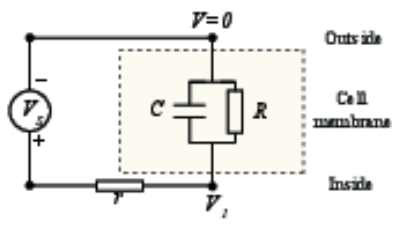
\includegraphics{pics/task1.png}
\caption{pic1}
\end{figure}

    At t=0 there is no voltage drop accros the capacitor and so it acts like
a shorted circuit, all the current flowing through it. As time goes on
there is more and more charge stored up, allowing less and less current
to flow through the capacitor and more through the resistor. After a
very long time when the capacitor is practically full, all the current
is flowing through the resistor. This is assuming Vs is constant.

    \hypertarget{choose-a-pulse}{%
\section{Choose a pulse}\label{choose-a-pulse}}

    \begin{tcolorbox}[breakable, size=fbox, boxrule=1pt, pad at break*=1mm,colback=cellbackground, colframe=cellborder]
\prompt{In}{incolor}{44}{\boxspacing}
\begin{Verbatim}[commandchars=\\\{\}]
\PY{c+c1}{\PYZsh{}a sinusoidal wave}
\PY{k+kn}{import} \PY{n+nn}{numpy} \PY{k}{as} \PY{n+nn}{np}


\PY{k}{def} \PY{n+nf}{Vpulse}\PY{p}{(}\PY{n}{t}\PY{p}{,} \PY{n}{t0}\PY{p}{,} \PY{n}{V0}\PY{p}{)}\PY{p}{:}
    \PY{k}{return} \PY{n}{V0}\PY{o}{*}\PY{n}{np}\PY{o}{.}\PY{n}{sin}\PY{p}{(}\PY{l+m+mi}{2}\PY{o}{*}\PY{n}{np}\PY{o}{.}\PY{n}{pi}\PY{o}{*}\PY{n}{t}\PY{o}{/}\PY{n}{t0}\PY{p}{)}
\end{Verbatim}
\end{tcolorbox}

    \begin{tcolorbox}[breakable, size=fbox, boxrule=1pt, pad at break*=1mm,colback=cellbackground, colframe=cellborder]
\prompt{In}{incolor}{2}{\boxspacing}
\begin{Verbatim}[commandchars=\\\{\}]
\PY{c+c1}{\PYZsh{}plot the wave}
\PY{k+kn}{import} \PY{n+nn}{matplotlib}\PY{n+nn}{.}\PY{n+nn}{pyplot} \PY{k}{as} \PY{n+nn}{pl}

\PY{n}{t} \PY{o}{=} \PY{n}{np}\PY{o}{.}\PY{n}{linspace}\PY{p}{(}\PY{l+m+mi}{0}\PY{p}{,} \PY{l+m+mf}{0.1}\PY{p}{,} \PY{l+m+mi}{1000}\PY{p}{)}
\PY{n}{t0} \PY{o}{=} \PY{l+m+mi}{1}\PY{o}{/}\PY{l+m+mi}{50} \PY{c+c1}{\PYZsh{} 50 Hz}
\PY{n}{Vs} \PY{o}{=} \PY{n}{Vpulse}\PY{p}{(}\PY{n}{t}\PY{p}{,} \PY{n}{t0}\PY{p}{,} \PY{l+m+mf}{230.0}\PY{p}{)}

\PY{n}{pl}\PY{o}{.}\PY{n}{plot}\PY{p}{(}\PY{n}{t}\PY{p}{,} \PY{n}{Vs}\PY{p}{)}
\PY{n}{pl}\PY{o}{.}\PY{n}{xlabel}\PY{p}{(}\PY{l+s+s2}{\PYZdq{}}\PY{l+s+s2}{time (s)}\PY{l+s+s2}{\PYZdq{}}\PY{p}{)}
\PY{n}{pl}\PY{o}{.}\PY{n}{ylabel}\PY{p}{(}\PY{l+s+s2}{\PYZdq{}}\PY{l+s+s2}{V}\PY{l+s+s2}{\PYZdq{}}\PY{p}{)}
\PY{n}{pl}\PY{o}{.}\PY{n}{show}\PY{p}{(}\PY{p}{)}
\end{Verbatim}
\end{tcolorbox}

    \begin{center}
    \adjustimage{max size={0.9\linewidth}{0.9\paperheight}}{output_5_0.png}
    \end{center}
    { \hspace*{\fill} \\}
    
    The wave can represent a signal from a wall socket.

    \hypertarget{study-the-propagation-of-the-pulse}{%
\section{Study the propagation of the
pulse}\label{study-the-propagation-of-the-pulse}}

    \begin{figure}
\centering
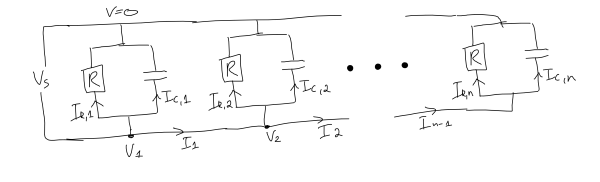
\includegraphics{pics/origsys.png}
\caption{os}
\end{figure}

    Vpulse(t) is the chosen sinusoidal wave. The code bellow uses the
numerical version of the cable equation to simulate the wave's
propagation through n elements pictured above. I will call them
elements.

    \begin{tcolorbox}[breakable, size=fbox, boxrule=1pt, pad at break*=1mm,colback=cellbackground, colframe=cellborder]
\prompt{In}{incolor}{42}{\boxspacing}
\begin{Verbatim}[commandchars=\\\{\}]
\PY{c+c1}{\PYZsh{} Initialize physical variables}
\PY{c+c1}{\PYZsh{} from oppgaveteksten}
\PY{n}{C} \PY{o}{=} \PY{l+m+mf}{1e\PYZhy{}10}
\PY{n}{R} \PY{o}{=} \PY{l+m+mf}{1e11}
\PY{n}{r} \PY{o}{=} \PY{l+m+mf}{1e6}
\PY{n}{V0} \PY{o}{=} \PY{l+m+mf}{100e\PYZhy{}3}

\PY{c+c1}{\PYZsh{} Set up simulation system}
\PY{n}{t0} \PY{o}{=} \PY{l+m+mi}{1}\PY{o}{/}\PY{l+m+mi}{50}

\PY{n}{resolution} \PY{o}{=} \PY{l+m+mi}{1000}
\PY{n}{dt} \PY{o}{=} \PY{n}{t0} \PY{o}{/} \PY{n}{resolution}
\PY{n}{time} \PY{o}{=} \PY{l+m+mf}{0.1}

\PY{c+c1}{\PYZsh{} Set up arrays for t and V[j,i]}
\PY{n}{n} \PY{o}{=} \PY{n+nb}{int}\PY{p}{(}\PY{n}{time} \PY{o}{/} \PY{n}{dt}\PY{p}{)}

\PY{c+c1}{\PYZsh{} a chain of 100 elements simulated for 10 waves}
\PY{n}{nrElem} \PY{o}{=} \PY{l+m+mi}{100}
\PY{n}{V} \PY{o}{=} \PY{n}{np}\PY{o}{.}\PY{n}{zeros}\PY{p}{(}\PY{p}{(}\PY{n}{n}\PY{p}{,} \PY{n}{nrElem}\PY{p}{)}\PY{p}{,} \PY{n+nb}{float}\PY{p}{)}
\PY{n}{t} \PY{o}{=} \PY{n}{np}\PY{o}{.}\PY{n}{zeros}\PY{p}{(}\PY{p}{(}\PY{n}{n}\PY{p}{,} \PY{l+m+mi}{1}\PY{p}{)}\PY{p}{,} \PY{n+nb}{float}\PY{p}{)}


\PY{c+c1}{\PYZsh{} Simulation loops : find V[j,i] for j = 1,2,3,..}


\PY{c+c1}{\PYZsh{} all elements are shorted at t=0}
\PY{c+c1}{\PYZsh{} because the current flows freely through the capacitors}
\PY{c+c1}{\PYZsh{} so their V is left being 0}

\PY{c+c1}{\PYZsh{} the first one is the voltage source unaffected by others}
\PY{n}{V}\PY{p}{[}\PY{l+m+mi}{0}\PY{p}{,} \PY{l+m+mi}{0}\PY{p}{]} \PY{o}{=} \PY{n}{Vpulse}\PY{p}{(}\PY{l+m+mi}{0}\PY{p}{,} \PY{n}{t0}\PY{p}{,} \PY{n}{V0}\PY{p}{)}

\PY{k}{for} \PY{n}{j} \PY{o+ow}{in} \PY{n+nb}{range}\PY{p}{(}\PY{n}{n} \PY{o}{\PYZhy{}} \PY{l+m+mi}{1}\PY{p}{)}\PY{p}{:}

    \PY{c+c1}{\PYZsh{} time += dt}
    \PY{n}{t}\PY{p}{[}\PY{n}{j} \PY{o}{+} \PY{l+m+mi}{1}\PY{p}{]} \PY{o}{=} \PY{n}{t}\PY{p}{[}\PY{n}{j}\PY{p}{]} \PY{o}{+} \PY{n}{dt}

    \PY{c+c1}{\PYZsh{} left\PYZhy{}most element where the signal starts}
    \PY{n}{V}\PY{p}{[}\PY{n}{j} \PY{o}{+} \PY{l+m+mi}{1}\PY{p}{,} \PY{l+m+mi}{0}\PY{p}{]} \PY{o}{=} \PY{n}{Vpulse}\PY{p}{(}\PY{n}{t}\PY{p}{[}\PY{n}{j} \PY{o}{+} \PY{l+m+mi}{1}\PY{p}{]}\PY{p}{,} \PY{n}{t0}\PY{p}{,} \PY{n}{V0}\PY{p}{)}

    \PY{c+c1}{\PYZsh{} all the others except the last}
    \PY{k}{for} \PY{n}{i} \PY{o+ow}{in} \PY{n+nb}{range}\PY{p}{(}\PY{l+m+mi}{1}\PY{p}{,} \PY{n}{nrElem} \PY{o}{\PYZhy{}} \PY{l+m+mi}{1}\PY{p}{)}\PY{p}{:}
        \PY{n}{V}\PY{p}{[}\PY{n}{j} \PY{o}{+} \PY{l+m+mi}{1}\PY{p}{,} \PY{n}{i}\PY{p}{]} \PY{o}{=} \PY{n}{V}\PY{p}{[}\PY{n}{j}\PY{p}{,} \PY{n}{i}\PY{p}{]} \PY{o}{+} \PY{n}{dt} \PY{o}{*} \PY{p}{(}
            \PY{p}{(}\PY{n}{V}\PY{p}{[}\PY{n}{j}\PY{p}{,} \PY{n}{i} \PY{o}{+} \PY{l+m+mi}{1}\PY{p}{]} \PY{o}{\PYZhy{}} \PY{l+m+mi}{2} \PY{o}{*} \PY{n}{V}\PY{p}{[}\PY{n}{j}\PY{p}{,} \PY{n}{i}\PY{p}{]} \PY{o}{+} \PY{n}{V}\PY{p}{[}\PY{n}{j}\PY{p}{,} \PY{n}{i} \PY{o}{\PYZhy{}} \PY{l+m+mi}{1}\PY{p}{]}\PY{p}{)} \PY{o}{/} \PY{p}{(}\PY{n}{r} \PY{o}{*} \PY{n}{C}\PY{p}{)} \PY{o}{\PYZhy{}} \PY{n}{V}\PY{p}{[}\PY{n}{j}\PY{p}{,} \PY{n}{i}\PY{p}{]} \PY{o}{/} \PY{p}{(}\PY{n}{R} \PY{o}{*} \PY{n}{C}\PY{p}{)}
        \PY{p}{)}

    \PY{c+c1}{\PYZsh{} last element}
    \PY{n}{i} \PY{o}{=} \PY{n}{nrElem} \PY{o}{\PYZhy{}} \PY{l+m+mi}{1}
    \PY{n}{V}\PY{p}{[}\PY{n}{j} \PY{o}{+} \PY{l+m+mi}{1}\PY{p}{,} \PY{n}{i}\PY{p}{]} \PY{o}{=} \PY{n}{V}\PY{p}{[}\PY{n}{j}\PY{p}{,} \PY{n}{i}\PY{p}{]} \PY{o}{+} \PY{n}{dt} \PY{o}{*} \PY{p}{(}\PY{p}{(}\PY{n}{V}\PY{p}{[}\PY{n}{j}\PY{p}{,} \PY{n}{i} \PY{o}{\PYZhy{}} \PY{l+m+mi}{1}\PY{p}{]} \PY{o}{\PYZhy{}} \PY{n}{V}\PY{p}{[}\PY{n}{j}\PY{p}{,} \PY{n}{i}\PY{p}{]}\PY{p}{)} \PY{o}{/} \PY{p}{(}\PY{n}{r} \PY{o}{*} \PY{n}{C}\PY{p}{)} \PY{o}{\PYZhy{}} \PY{n}{V}\PY{p}{[}\PY{n}{j}\PY{p}{,} \PY{n}{i}\PY{p}{]} \PY{o}{/} \PY{p}{(}\PY{n}{R} \PY{o}{*} \PY{n}{C}\PY{p}{)}\PY{p}{)}
\end{Verbatim}
\end{tcolorbox}

    Here I study how the voltage changes over time for elements close to the
source, in the middle and at the end of the chain.

    \begin{tcolorbox}[breakable, size=fbox, boxrule=1pt, pad at break*=1mm,colback=cellbackground, colframe=cellborder]
\prompt{In}{incolor}{43}{\boxspacing}
\begin{Verbatim}[commandchars=\\\{\}]
\PY{c+c1}{\PYZsh{}close to the source}

\PY{n}{pl}\PY{o}{.}\PY{n}{figure}\PY{p}{(}\PY{n}{figsize}\PY{o}{=}\PY{p}{(}\PY{l+m+mi}{10}\PY{p}{,} \PY{l+m+mi}{6}\PY{p}{)}\PY{p}{)}

\PY{n}{pl}\PY{o}{.}\PY{n}{subplot}\PY{p}{(}\PY{l+m+mi}{311}\PY{p}{)}
\PY{k}{for} \PY{n}{j} \PY{o+ow}{in} \PY{p}{[}\PY{l+m+mi}{0}\PY{p}{,} \PY{l+m+mi}{2}\PY{p}{,} \PY{l+m+mi}{7}\PY{p}{]}\PY{p}{:}
    \PY{n}{pl}\PY{o}{.}\PY{n}{plot}\PY{p}{(}\PY{n}{t}\PY{p}{,} \PY{n}{V}\PY{p}{[}\PY{p}{:}\PY{p}{,} \PY{n}{j}\PY{p}{]}\PY{p}{,} \PY{n}{label}\PY{o}{=}\PY{l+s+sa}{f}\PY{l+s+s2}{\PYZdq{}}\PY{l+s+s2}{nr }\PY{l+s+si}{\PYZob{}j\PYZcb{}}\PY{l+s+s2}{\PYZdq{}}\PY{p}{)}
\PY{n}{pl}\PY{o}{.}\PY{n}{legend}\PY{p}{(}\PY{p}{)}\PY{p}{;} \PY{n}{pl}\PY{o}{.}\PY{n}{ylabel}\PY{p}{(}\PY{l+s+s2}{\PYZdq{}}\PY{l+s+s2}{V}\PY{l+s+s2}{\PYZdq{}}\PY{p}{)}\PY{p}{;} \PY{n}{pl}\PY{o}{.}\PY{n}{xlabel}\PY{p}{(}\PY{l+s+s2}{\PYZdq{}}\PY{l+s+s2}{time (s)}\PY{l+s+s2}{\PYZdq{}}\PY{p}{)}\PY{p}{;}

\PY{c+c1}{\PYZsh{}middle}
\PY{n}{pl}\PY{o}{.}\PY{n}{subplot}\PY{p}{(}\PY{l+m+mi}{312}\PY{p}{)}
\PY{k}{for} \PY{n}{j} \PY{o+ow}{in} \PY{p}{[}\PY{l+m+mi}{40}\PY{p}{,} \PY{l+m+mi}{45}\PY{p}{,} \PY{l+m+mi}{50}\PY{p}{]}\PY{p}{:}
    \PY{n}{pl}\PY{o}{.}\PY{n}{plot}\PY{p}{(}\PY{n}{t}\PY{p}{,} \PY{n}{V}\PY{p}{[}\PY{p}{:}\PY{p}{,} \PY{n}{j}\PY{p}{]}\PY{p}{,} \PY{n}{label}\PY{o}{=}\PY{l+s+sa}{f}\PY{l+s+s2}{\PYZdq{}}\PY{l+s+s2}{nr }\PY{l+s+si}{\PYZob{}j\PYZcb{}}\PY{l+s+s2}{\PYZdq{}}\PY{p}{)}
\PY{n}{pl}\PY{o}{.}\PY{n}{legend}\PY{p}{(}\PY{p}{)}\PY{p}{;} \PY{n}{pl}\PY{o}{.}\PY{n}{ylabel}\PY{p}{(}\PY{l+s+s2}{\PYZdq{}}\PY{l+s+s2}{V}\PY{l+s+s2}{\PYZdq{}}\PY{p}{)}\PY{p}{;} \PY{n}{pl}\PY{o}{.}\PY{n}{xlabel}\PY{p}{(}\PY{l+s+s2}{\PYZdq{}}\PY{l+s+s2}{time (s)}\PY{l+s+s2}{\PYZdq{}}\PY{p}{)}\PY{p}{;}

\PY{c+c1}{\PYZsh{}end}
\PY{n}{pl}\PY{o}{.}\PY{n}{subplot}\PY{p}{(}\PY{l+m+mi}{313}\PY{p}{)}
\PY{k}{for} \PY{n}{j} \PY{o+ow}{in} \PY{p}{[}\PY{l+m+mi}{75}\PY{p}{,} \PY{l+m+mi}{85}\PY{p}{,} \PY{l+m+mi}{90}\PY{p}{]}\PY{p}{:}
    \PY{n}{pl}\PY{o}{.}\PY{n}{plot}\PY{p}{(}\PY{n}{t}\PY{p}{,} \PY{n}{V}\PY{p}{[}\PY{p}{:}\PY{p}{,} \PY{n}{j}\PY{p}{]}\PY{p}{,} \PY{n}{label}\PY{o}{=}\PY{l+s+sa}{f}\PY{l+s+s2}{\PYZdq{}}\PY{l+s+s2}{nr }\PY{l+s+si}{\PYZob{}j\PYZcb{}}\PY{l+s+s2}{\PYZdq{}}\PY{p}{)}
\PY{n}{pl}\PY{o}{.}\PY{n}{legend}\PY{p}{(}\PY{p}{)}\PY{p}{;} \PY{n}{pl}\PY{o}{.}\PY{n}{ylabel}\PY{p}{(}\PY{l+s+s2}{\PYZdq{}}\PY{l+s+s2}{V}\PY{l+s+s2}{\PYZdq{}}\PY{p}{)}\PY{p}{;} \PY{n}{pl}\PY{o}{.}\PY{n}{xlabel}\PY{p}{(}\PY{l+s+s2}{\PYZdq{}}\PY{l+s+s2}{time (s)}\PY{l+s+s2}{\PYZdq{}}\PY{p}{)}\PY{p}{;}


\PY{n}{pl}\PY{o}{.}\PY{n}{show}\PY{p}{(}\PY{p}{)}
\end{Verbatim}
\end{tcolorbox}

    \begin{center}
    \adjustimage{max size={0.9\linewidth}{0.9\paperheight}}{output_12_0.png}
    \end{center}
    { \hspace*{\fill} \\}
    
    I can see the the farther away we get from the source the lower the
voltage over the element. The ones close to the source seem stable and
predictable. And the closer we get to the source the more like the
source the voltage gets. They dont seem to decay over time. If we look
at nr 7 there is a delay in when it peaks, but the number of peaks is
the same. And the farther away we move the greater the delay.

Now those in the middle are visibly decaying over time. Again, with the
voltage getting lower and delay greater the farther away the element is.
But the absolute decay is bigger for nr 40 than it is for nr 50. And it
appears the voltage never gets negative unlike the original signal.

And as we move to the end of the chain the voltage is flatter and
flatter and the voltage on nr 85 and 90 is still rising. Still
increasing the (average) charge in their capacitors. Nr 75 is at its
peak, and if it follows the pattern it will start to decay. At the end
there it is coming down from a local peak, because of the wave, but that
doesnt really tell us anything about the trend farther in time. Looking
at number 90 it is hard to tell that the original voltage source is a
sinusoidal wave.

    \hypertarget{modify-the-model}{%
\section{Modify the model}\label{modify-the-model}}

    In this project we modify the cable equation of a cell membrane to
include the effect of a voltage-gated resistor instead of a regular one.

    \begin{figure}
\centering
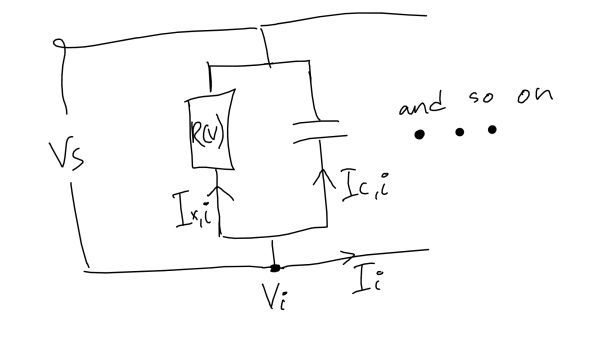
\includegraphics{pics/Task4sys.png}
\caption{ts4}
\end{figure}

    This changes \(I_x\) in the original expression we used to find the next
element Vj+1.

    \begin{figure}
\centering
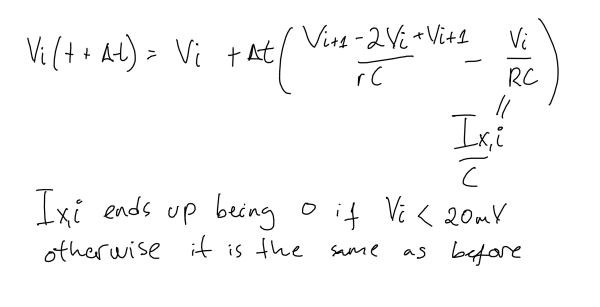
\includegraphics{pics/task4i.png}
\caption{ts4i}
\end{figure}

    For N=1 immediately after the signal turns on the current flows through
the capacitor as before with no resitance and R(v) is infinite(no
current). After a short while when there is enough charge in the
capacitor and the voltage exceeds 20mV, R(v) becomes just plain R and
current starts flowing through it as well and the system acts in the
same way as it did before. When the signal switches direction
(sinusoidal pulse) the capacitor will get discharged at one point and
the voltage will drop bellow 20mV. And so it will loop.

    Code to simulate the propagation is the same as before with minor
adjustments.

    \begin{tcolorbox}[breakable, size=fbox, boxrule=1pt, pad at break*=1mm,colback=cellbackground, colframe=cellborder]
\prompt{In}{incolor}{64}{\boxspacing}
\begin{Verbatim}[commandchars=\\\{\}]
\PY{c+c1}{\PYZsh{} Initialize physical variables}
\PY{c+c1}{\PYZsh{} from oppgaveteksten}
\PY{n}{C} \PY{o}{=} \PY{l+m+mf}{1e\PYZhy{}10}
\PY{n}{R} \PY{o}{=} \PY{l+m+mf}{1e11}
\PY{n}{r} \PY{o}{=} \PY{l+m+mf}{1e6}
\PY{n}{V0} \PY{o}{=} \PY{l+m+mf}{100e\PYZhy{}3}

\PY{c+c1}{\PYZsh{} Set up simulation system}
\PY{n}{t0} \PY{o}{=} \PY{l+m+mi}{1}\PY{o}{/}\PY{l+m+mi}{50}

\PY{n}{resolution} \PY{o}{=} \PY{l+m+mi}{1000}
\PY{n}{dt} \PY{o}{=} \PY{n}{t0} \PY{o}{/} \PY{n}{resolution}
\PY{n}{time} \PY{o}{=} \PY{l+m+mf}{0.1}

\PY{c+c1}{\PYZsh{} Set up arrays for t and V[j,i]}
\PY{n}{n} \PY{o}{=} \PY{n+nb}{int}\PY{p}{(}\PY{n}{time} \PY{o}{/} \PY{n}{dt}\PY{p}{)}

\PY{c+c1}{\PYZsh{} a chain of 100 elements simulated for 10 waves}
\PY{n}{nrElem} \PY{o}{=} \PY{l+m+mi}{100}
\PY{n}{V} \PY{o}{=} \PY{n}{np}\PY{o}{.}\PY{n}{zeros}\PY{p}{(}\PY{p}{(}\PY{n}{n}\PY{p}{,} \PY{n}{nrElem}\PY{p}{)}\PY{p}{,} \PY{n+nb}{float}\PY{p}{)}
\PY{n}{t} \PY{o}{=} \PY{n}{np}\PY{o}{.}\PY{n}{zeros}\PY{p}{(}\PY{p}{(}\PY{n}{n}\PY{p}{,} \PY{l+m+mi}{1}\PY{p}{)}\PY{p}{,} \PY{n+nb}{float}\PY{p}{)}


\PY{c+c1}{\PYZsh{} Simulation loops : find V[j,i] for j = 1,2,3,..}


\PY{c+c1}{\PYZsh{} all elements are shorted at t=0}
\PY{c+c1}{\PYZsh{} because the current flows freely through the capacitors}
\PY{c+c1}{\PYZsh{} so their V is left being 0}

\PY{c+c1}{\PYZsh{} the first one is the voltage source unaffected by others}
\PY{n}{V}\PY{p}{[}\PY{l+m+mi}{0}\PY{p}{,} \PY{l+m+mi}{0}\PY{p}{]} \PY{o}{=} \PY{n}{Vpulse}\PY{p}{(}\PY{l+m+mi}{0}\PY{p}{,} \PY{n}{t0}\PY{p}{,} \PY{n}{V0}\PY{p}{)}

\PY{k}{for} \PY{n}{j} \PY{o+ow}{in} \PY{n+nb}{range}\PY{p}{(}\PY{n}{n} \PY{o}{\PYZhy{}} \PY{l+m+mi}{1}\PY{p}{)}\PY{p}{:}

    \PY{c+c1}{\PYZsh{} time += dt}
    \PY{n}{t}\PY{p}{[}\PY{n}{j} \PY{o}{+} \PY{l+m+mi}{1}\PY{p}{]} \PY{o}{=} \PY{n}{t}\PY{p}{[}\PY{n}{j}\PY{p}{]} \PY{o}{+} \PY{n}{dt}

    \PY{c+c1}{\PYZsh{} left\PYZhy{}most element where the signal starts}
    \PY{n}{V}\PY{p}{[}\PY{n}{j} \PY{o}{+} \PY{l+m+mi}{1}\PY{p}{,} \PY{l+m+mi}{0}\PY{p}{]} \PY{o}{=} \PY{n}{Vpulse}\PY{p}{(}\PY{n}{t}\PY{p}{[}\PY{n}{j} \PY{o}{+} \PY{l+m+mi}{1}\PY{p}{]}\PY{p}{,} \PY{n}{t0}\PY{p}{,} \PY{n}{V0}\PY{p}{)}
    

    \PY{c+c1}{\PYZsh{} all the others except the last}
    \PY{k}{for} \PY{n}{i} \PY{o+ow}{in} \PY{n+nb}{range}\PY{p}{(}\PY{l+m+mi}{1}\PY{p}{,} \PY{n}{nrElem} \PY{o}{\PYZhy{}} \PY{l+m+mi}{1}\PY{p}{)}\PY{p}{:}
        \PY{c+c1}{\PYZsh{}the change}
        \PY{n}{Ixi} \PY{o}{=} \PY{p}{(}\PY{n}{V}\PY{p}{[}\PY{n}{j}\PY{p}{,} \PY{n}{i}\PY{p}{]} \PY{o}{/} \PY{n}{R}\PY{p}{)} \PY{k}{if} \PY{p}{(}\PY{n}{V}\PY{p}{[}\PY{n}{j}\PY{p}{,} \PY{n}{i}\PY{p}{]} \PY{o}{\PYZgt{}}\PY{o}{=} \PY{l+m+mf}{20e\PYZhy{}3}\PY{p}{)} \PY{k}{else} \PY{l+m+mi}{0}
        
        \PY{n}{V}\PY{p}{[}\PY{n}{j} \PY{o}{+} \PY{l+m+mi}{1}\PY{p}{,} \PY{n}{i}\PY{p}{]} \PY{o}{=} \PY{n}{V}\PY{p}{[}\PY{n}{j}\PY{p}{,} \PY{n}{i}\PY{p}{]} \PY{o}{+} \PY{n}{dt} \PY{o}{*} \PY{p}{(}
            \PY{p}{(}\PY{n}{V}\PY{p}{[}\PY{n}{j}\PY{p}{,} \PY{n}{i} \PY{o}{+} \PY{l+m+mi}{1}\PY{p}{]} \PY{o}{\PYZhy{}} \PY{l+m+mi}{2} \PY{o}{*} \PY{n}{V}\PY{p}{[}\PY{n}{j}\PY{p}{,} \PY{n}{i}\PY{p}{]} \PY{o}{+} \PY{n}{V}\PY{p}{[}\PY{n}{j}\PY{p}{,} \PY{n}{i} \PY{o}{\PYZhy{}} \PY{l+m+mi}{1}\PY{p}{]}\PY{p}{)} \PY{o}{/} \PY{p}{(}\PY{n}{r} \PY{o}{*} \PY{n}{C}\PY{p}{)} \PY{o}{\PYZhy{}} \PY{n}{Ixi}\PY{o}{/}\PY{n}{C}
        \PY{p}{)}

    \PY{c+c1}{\PYZsh{} last element}
    \PY{n}{i} \PY{o}{=} \PY{n}{nrElem} \PY{o}{\PYZhy{}} \PY{l+m+mi}{1}
    \PY{n}{Ixi} \PY{o}{=} \PY{p}{(}\PY{n}{V}\PY{p}{[}\PY{n}{j}\PY{p}{,} \PY{n}{i}\PY{p}{]} \PY{o}{/} \PY{n}{R}\PY{p}{)} \PY{k}{if} \PY{p}{(}\PY{n}{V}\PY{p}{[}\PY{n}{j}\PY{p}{,} \PY{n}{i}\PY{p}{]} \PY{o}{\PYZgt{}}\PY{o}{=} \PY{l+m+mf}{20e\PYZhy{}3}\PY{p}{)} \PY{k}{else} \PY{l+m+mi}{0}
    \PY{n}{V}\PY{p}{[}\PY{n}{j} \PY{o}{+} \PY{l+m+mi}{1}\PY{p}{,} \PY{n}{i}\PY{p}{]} \PY{o}{=} \PY{n}{V}\PY{p}{[}\PY{n}{j}\PY{p}{,} \PY{n}{i}\PY{p}{]} \PY{o}{+} \PY{n}{dt} \PY{o}{*} \PY{p}{(}\PY{p}{(}\PY{n}{V}\PY{p}{[}\PY{n}{j}\PY{p}{,} \PY{n}{i} \PY{o}{\PYZhy{}} \PY{l+m+mi}{1}\PY{p}{]} \PY{o}{\PYZhy{}} \PY{n}{V}\PY{p}{[}\PY{n}{j}\PY{p}{,} \PY{n}{i}\PY{p}{]}\PY{p}{)} \PY{o}{/} \PY{p}{(}\PY{n}{r} \PY{o}{*} \PY{n}{C}\PY{p}{)} \PY{o}{\PYZhy{}} \PY{n}{Ixi}\PY{o}{/}\PY{n}{C}\PY{p}{)}
\end{Verbatim}
\end{tcolorbox}

    Lets do the same plots as before so we can compare.

    \begin{tcolorbox}[breakable, size=fbox, boxrule=1pt, pad at break*=1mm,colback=cellbackground, colframe=cellborder]
\prompt{In}{incolor}{63}{\boxspacing}
\begin{Verbatim}[commandchars=\\\{\}]
\PY{n}{pl}\PY{o}{.}\PY{n}{figure}\PY{p}{(}\PY{n}{figsize}\PY{o}{=}\PY{p}{(}\PY{l+m+mi}{10}\PY{p}{,} \PY{l+m+mi}{6}\PY{p}{)}\PY{p}{)}

\PY{n}{pl}\PY{o}{.}\PY{n}{subplot}\PY{p}{(}\PY{l+m+mi}{311}\PY{p}{)}
\PY{k}{for} \PY{n}{j} \PY{o+ow}{in} \PY{p}{[}\PY{l+m+mi}{0}\PY{p}{,} \PY{l+m+mi}{2}\PY{p}{,} \PY{l+m+mi}{7}\PY{p}{]}\PY{p}{:}
    \PY{n}{pl}\PY{o}{.}\PY{n}{plot}\PY{p}{(}\PY{n}{t}\PY{p}{,} \PY{n}{V}\PY{p}{[}\PY{p}{:}\PY{p}{,} \PY{n}{j}\PY{p}{]}\PY{p}{,} \PY{n}{label}\PY{o}{=}\PY{l+s+sa}{f}\PY{l+s+s2}{\PYZdq{}}\PY{l+s+s2}{nr }\PY{l+s+si}{\PYZob{}j\PYZcb{}}\PY{l+s+s2}{\PYZdq{}}\PY{p}{)}
\PY{n}{pl}\PY{o}{.}\PY{n}{legend}\PY{p}{(}\PY{p}{)}\PY{p}{;} \PY{n}{pl}\PY{o}{.}\PY{n}{ylabel}\PY{p}{(}\PY{l+s+s2}{\PYZdq{}}\PY{l+s+s2}{V}\PY{l+s+s2}{\PYZdq{}}\PY{p}{)}\PY{p}{;} \PY{n}{pl}\PY{o}{.}\PY{n}{xlabel}\PY{p}{(}\PY{l+s+s2}{\PYZdq{}}\PY{l+s+s2}{time (s)}\PY{l+s+s2}{\PYZdq{}}\PY{p}{)}\PY{p}{;}

\PY{c+c1}{\PYZsh{}middle}
\PY{n}{pl}\PY{o}{.}\PY{n}{subplot}\PY{p}{(}\PY{l+m+mi}{312}\PY{p}{)}
\PY{k}{for} \PY{n}{j} \PY{o+ow}{in} \PY{p}{[}\PY{l+m+mi}{40}\PY{p}{,} \PY{l+m+mi}{45}\PY{p}{,} \PY{l+m+mi}{50}\PY{p}{]}\PY{p}{:}
    \PY{n}{pl}\PY{o}{.}\PY{n}{plot}\PY{p}{(}\PY{n}{t}\PY{p}{,} \PY{n}{V}\PY{p}{[}\PY{p}{:}\PY{p}{,} \PY{n}{j}\PY{p}{]}\PY{p}{,} \PY{n}{label}\PY{o}{=}\PY{l+s+sa}{f}\PY{l+s+s2}{\PYZdq{}}\PY{l+s+s2}{nr }\PY{l+s+si}{\PYZob{}j\PYZcb{}}\PY{l+s+s2}{\PYZdq{}}\PY{p}{)}
\PY{n}{pl}\PY{o}{.}\PY{n}{legend}\PY{p}{(}\PY{p}{)}\PY{p}{;} \PY{n}{pl}\PY{o}{.}\PY{n}{ylabel}\PY{p}{(}\PY{l+s+s2}{\PYZdq{}}\PY{l+s+s2}{V}\PY{l+s+s2}{\PYZdq{}}\PY{p}{)}\PY{p}{;} \PY{n}{pl}\PY{o}{.}\PY{n}{xlabel}\PY{p}{(}\PY{l+s+s2}{\PYZdq{}}\PY{l+s+s2}{time (s)}\PY{l+s+s2}{\PYZdq{}}\PY{p}{)}\PY{p}{;}

\PY{c+c1}{\PYZsh{}end}
\PY{n}{pl}\PY{o}{.}\PY{n}{subplot}\PY{p}{(}\PY{l+m+mi}{313}\PY{p}{)}
\PY{k}{for} \PY{n}{j} \PY{o+ow}{in} \PY{p}{[}\PY{l+m+mi}{75}\PY{p}{,} \PY{l+m+mi}{85}\PY{p}{,} \PY{l+m+mi}{90}\PY{p}{]}\PY{p}{:}
    \PY{n}{pl}\PY{o}{.}\PY{n}{plot}\PY{p}{(}\PY{n}{t}\PY{p}{,} \PY{n}{V}\PY{p}{[}\PY{p}{:}\PY{p}{,} \PY{n}{j}\PY{p}{]}\PY{p}{,} \PY{n}{label}\PY{o}{=}\PY{l+s+sa}{f}\PY{l+s+s2}{\PYZdq{}}\PY{l+s+s2}{nr }\PY{l+s+si}{\PYZob{}j\PYZcb{}}\PY{l+s+s2}{\PYZdq{}}\PY{p}{)}
\PY{n}{pl}\PY{o}{.}\PY{n}{legend}\PY{p}{(}\PY{p}{)}\PY{p}{;} \PY{n}{pl}\PY{o}{.}\PY{n}{ylabel}\PY{p}{(}\PY{l+s+s2}{\PYZdq{}}\PY{l+s+s2}{V}\PY{l+s+s2}{\PYZdq{}}\PY{p}{)}\PY{p}{;} \PY{n}{pl}\PY{o}{.}\PY{n}{xlabel}\PY{p}{(}\PY{l+s+s2}{\PYZdq{}}\PY{l+s+s2}{time (s)}\PY{l+s+s2}{\PYZdq{}}\PY{p}{)}\PY{p}{;}


\PY{n}{pl}\PY{o}{.}\PY{n}{show}\PY{p}{(}\PY{p}{)}
\end{Verbatim}
\end{tcolorbox}

    \begin{center}
    \adjustimage{max size={0.9\linewidth}{0.9\paperheight}}{output_23_0.png}
    \end{center}
    { \hspace*{\fill} \\}
    
    There is no obvious difference between the models. One would expect that
current not leaking through the R but rather filling up the capacitor
faster would cause some change. But no. So everything mentioned above
for the original model applies here.


    % Add a bibliography block to the postdoc
    
    
    
\end{document}
